\chapter{Project Management and Design}

Chapter~1 explained \emph{what} the platform is and \emph{why} it exists. This chapter explains
\emph{how} the project was planned before implementation began. It covers the development
methodology, the product backlog and the non-functional requirements, the sprint plan, the
software architecture, the database design, the technology choices, the testing strategy, and the
expected risks and challenges. The five development sprints are described in Chapters~3 and~4, and
the AI sprint in Chapter~5.

\section{Development Methodology}

This section explains how the project was run: the method that was chosen, the team roles, and
how the sprints were organized.

\subsection{Why Scrum}

We adopted \textbf{Scrum}~\cite{schwaber2020scrum} as the development methodology. The choice
comes from the nature of the work itself. The platform covers ten operational domains (as
described in Section~1.6.3), and the requirements for the later ones --- notifications,
monitoring, and above all the AI copilot --- could only become clear after the earlier ones
were built and used. A single up-front waterfall specification would have fixed decisions too
early, before we had the knowledge to make them. Scrum allowed us to deliver the platform in
working increments: first the authentication core, then projects on top of it, then the agile
backlog on top of projects. Each increment could be demonstrated, and the next one was planned
against a working system.

\subsection{Scrum roles}

The work was organized as a three-person Scrum team:

\begin{itemize}
  \item \textbf{Aymen BenHsan} (the author) --- Development Team and main developer, responsible
    for the full-stack design and implementation.
  \item \textbf{Ahmed Awedi} (CEO) --- Product Owner and frontend supervisor, owning priorities
    and the product backlog.
  \item \textbf{Mohamed Awedi} (CTO) --- Backend supervisor, providing technical guidance and
    unblocking.
\end{itemize}

\subsection{Sprint organization}

Each sprint followed the standard Scrum ceremonies:

\begin{itemize}
  \item \textbf{Sprint planning}: select a set of user stories from the product backlog into the
    sprint backlog and agree on a sprint goal.
  \item \textbf{Daily stand-ups}: short synchronization meetings.
  \item \textbf{Sprint review}: demo the delivered increment.
  \item \textbf{Retrospective}: improve the process for the next sprint.
  \item \textbf{Backlog refinement}: ran continuously as the later domains became clearer.
\end{itemize}

Each sprint produced three artifacts: a \textbf{sprint backlog} drawn from the product backlog, a
\textbf{sprint goal} defining the target, and a potentially shippable \textbf{increment}.

\subsection{Sprint duration}

Sprint durations were \textbf{variable}, adjusted to the scope and complexity of each sprint's
backlog rather than fixed at a uniform length. Sprints ranged from two weeks (Sprint~2, the
lightest) to five weeks (Sprint~3, the heaviest at 64 story points). The total project timeline
spans the five-month internship period (February--July 2026).

\subsection{Methodological note}

The sprint boundaries follow the system's module dependency order, because that order was not a
choice: authentication had to exist before projects could be scoped to a user, projects before
the agile backlog could attach to anything, and the content of all five earlier sprints before a
copilot could index it. Each sprint therefore closes on the smallest increment that leaves the
platform in a demonstrable state, which is also what made the review at the end of each one
meaningful.

One additional note: inside Sprint~6, where the RAG copilot is built, we use a second
methodology as a sub-process --- \textbf{CRISP-DM}~\cite{shearer2000crisp} (Cross-Industry
Standard Process for Data Mining). An ML component needs steps that ordinary CRUD features do
not: data understanding, modeling, and evaluation. This is detailed in Chapter~5.

\section{Product Backlog}

The backlog expresses each delivered module's endpoints and features as user stories in the
canonical \emph{``As a <role>, I want <goal>, so that <value>''} form. Story identifiers are
stable and sprint-scoped (\texttt{US-S<sprint>-<n>}). Priority uses MoSCoW (\textbf{Must / Should
/ Could}). Story points use a Fibonacci scale (1, 2, 3, 5, 8) as a relative size and complexity
estimate. Estimated durations are derived from the sprint timeline and story-point proportions.

\subsection{Sprint 1 --- Foundations \& Authentication}

\begin{longtable}{@{}l>{\raggedright\arraybackslash}p{0.50\textwidth}lll@{}}
\caption{Sprint 1 backlog.}\label{tab:sprint1-backlog} \\
\tableheaderrow
\thcell{US-ID} & \thcell{Story} & \thcell{SP} & \thcell{Est.} & \thcell{Priority} \\
\midrule
\endfirsthead
\caption[]{Sprint 1 backlog (continued).} \\
\tableheaderrow
\thcell{US-ID} & \thcell{Story} & \thcell{SP} & \thcell{Est.} & \thcell{Priority} \\
\midrule
\endhead
\bottomrule
\endfoot
US-S1-01 & As a developer, I want a layered NestJS backend with a Prisma multi-file schema and migrations, so that every module shares one structure. & 8 & 4d & Must \\
\midrule
US-S1-02 & As a user, I want to log in with email + password and receive a JWT, so that I can access the platform. & 3 & 1.5d & Must \\
\midrule
US-S1-03 & As a user, I want my session refreshed automatically on expiry, so that I stay logged in without re-authenticating. & 3 & 1d & Must \\
\midrule
US-S1-04 & As a user, I want to reset a forgotten password via an emailed code, so that I can regain access. & 3 & 2d & Should \\
\midrule
US-S1-05 & As the platform, I want every protected endpoint gated by a role-permission guard, so that a user only reaches what their role allows. & 8 & 3.5d & Must \\
\midrule
US-S1-06 & As an admin/HR, I want to provision user accounts directly with one or more roles, so that staff can be onboarded immediately without going through self-registration's pending-approval step. & 5 & 2.5d & Must \\
\midrule
US-S1-07 & As an admin, I want to list, search (accent-insensitive), and filter users, so that I can manage the directory. & 3 & 1.5d & Should \\
\midrule
US-S1-08 & As an admin, I want to edit and soft-delete (deactivate) a user, so that I manage the account lifecycle. & 3 & 1.5d & Must \\
\midrule
US-S1-09 & As a user, I want to update my own profile and change my password, so that I manage my account. & 2 & 1d & Should \\
\midrule
US-S1-10 & As an admin, I want to create teams and assign members and a manager, so that staff are grouped. & 3 & 1.5d & Should \\
\midrule
& \textbf{Sprint 1 subtotal} & \textbf{41} & \textbf{3w} & \\
\end{longtable}

\subsection{Sprint 2 --- Projects \& Membership}

\begin{longtable}{@{}l>{\raggedright\arraybackslash}p{0.50\textwidth}lll@{}}
\caption{Sprint 2 backlog.}\label{tab:sprint2-backlog} \\
\tableheaderrow
\thcell{US-ID} & \thcell{Story} & \thcell{SP} & \thcell{Est.} & \thcell{Priority} \\
\midrule
\endfirsthead
\caption[]{Sprint 2 backlog (continued).} \\
\tableheaderrow
\thcell{US-ID} & \thcell{Story} & \thcell{SP} & \thcell{Est.} & \thcell{Priority} \\
\midrule
\endhead
\bottomrule
\endfoot
US-S2-01 & As a manager/executive, I want to create a project under a business unit with a type (AGILE/FREESTYLE), so that work is organized by unit and workflow. & 5 & 2.5d & Must \\
\midrule
US-S2-02 & As a manager, I want to edit, archive, and delete a project, so that I manage its lifecycle. & 3 & 1.5d & Must \\
\midrule
US-S2-03 & As a manager, I want to add existing users as project members and mark a manager, so that the team is defined. & 3 & 1.5d & Must \\
\midrule
US-S2-04 & As a manager, I want to invite people by email with a single-use token, so that non-members can be brought in. & 5 & 3d & Should \\
\midrule
US-S2-05 & As an invitee, I want to accept an emailed invitation, so that I become a member. & 3 & 1.5d & Should \\
\midrule
US-S2-06 & As a manager, I want to configure the project's kanban settings (WIP limits), so that the board fits our process. & 2 & 1d & Could \\
\midrule
US-S2-07 & As a member, I want to see only the projects I belong to (executives scoped to their business unit), so that access is isolated. & 5 & 2d & Must \\
\midrule
& \textbf{Sprint 2 subtotal} & \textbf{26} & \textbf{2w} & \\
\end{longtable}

\subsection{Sprint 3 --- Agile Backlog \& Tasks}

\begin{longtable}{@{}l>{\raggedright\arraybackslash}p{0.50\textwidth}lll@{}}
\caption{Sprint 3 backlog.}\label{tab:sprint3-backlog} \\
\tableheaderrow
\thcell{US-ID} & \thcell{Story} & \thcell{SP} & \thcell{Est.} & \thcell{Priority} \\
\midrule
\endfirsthead
\caption[]{Sprint 3 backlog (continued).} \\
\tableheaderrow
\thcell{US-ID} & \thcell{Story} & \thcell{SP} & \thcell{Est.} & \thcell{Priority} \\
\midrule
\endhead
\bottomrule
\endfoot
US-S3-01 & As a PM/PO, I want to create epics to group large features, so that the backlog is structured. & 3 & 1.5d & Should \\
\midrule
US-S3-02 & As a Scrum Master, I want to create sprints with dates and a capacity, so that work is time-boxed. & 5 & 3d & Must \\
\midrule
US-S3-03 & As a Scrum Master, I want to run the sprint lifecycle (start/stop/complete, one running at a time), so that iterations are governed. & 8 & 4d & Must \\
\midrule
US-S3-04 & As a PM, I want milestones with target dates (also for FREESTYLE projects), so that deadlines are tracked. & 3 & 1.5d & Should \\
\midrule
US-S3-05 & As a PM, I want burndown, velocity, and Gantt analytics, so that I can monitor progress. & 8 & 3.5d & Should \\
\midrule
US-S3-06 & As a member, I want to create tasks with type, priority, assignee, and estimates, so that work is captured. & 5 & 2.5d & Must \\
\midrule
US-S3-07 & As a manager, I want a per-project, data-driven kanban with custom columns and WIP limits, so that the board mirrors our workflow. & 8 & 4d & Must \\
\midrule
US-S3-08 & As an assignee, I want to move a task across columns with transition, dependency, and WIP validation, so that status stays valid. & 8 & 3.5d & Must \\
\midrule
US-S3-09 & As a member, I want to declare task dependencies (blocking / blocked-by), so that ordering is explicit. & 5 & 2d & Should \\
\midrule
US-S3-10 & As a member, I want to log time against a task, so that effort is recorded. & 3 & 1.5d & Should \\
\midrule
US-S3-11 & As a member, I want threaded comments with @mentions and likes on a task, so that we collaborate in context. & 5 & 2.5d & Should \\
\midrule
US-S3-12 & As a member, I want labels and to assign a task to a sprint/epic/milestone, so that work is categorized. & 3 & 1.5d & Should \\
\midrule
& \textbf{Sprint 3 subtotal} & \textbf{64} & \textbf{5w} & \\
\end{longtable}

\subsection{Sprint 4 --- Productivity Suite}

\begin{longtable}{@{}l>{\raggedright\arraybackslash}p{0.50\textwidth}lll@{}}
\caption{Sprint 4 backlog.}\label{tab:sprint4-backlog} \\
\tableheaderrow
\thcell{US-ID} & \thcell{Story} & \thcell{SP} & \thcell{Est.} & \thcell{Priority} \\
\midrule
\endfirsthead
\caption[]{Sprint 4 backlog (continued).} \\
\tableheaderrow
\thcell{US-ID} & \thcell{Story} & \thcell{SP} & \thcell{Est.} & \thcell{Priority} \\
\midrule
\endhead
\bottomrule
\endfoot
US-S4-01 & As a user, I want a private to-do list with sub-tasks, priorities, and statuses, so that I track my own work separately from project tasks. & 5 & 2.5d & Should \\
\midrule
US-S4-02 & As a user, I want due/reminder dates on my to-dos that notify me across my channels, so that nothing slips. & 5 & 2d & Should \\
\midrule
US-S4-03 & As an employee, I want to check in and out (remote/onsite) to open and close work sessions, so that attendance is recorded. & 8 & 4d & Must \\
\midrule
US-S4-04 & As an employee, I want my worked time computed per business day, so that I can see my hours. & 3 & 1.5d & Should \\
\midrule
US-S4-05 & As a manager, I want per-user and per-team attendance statistics, so that I can review presence. & 5 & 2.5d & Should \\
\midrule
US-S4-06 & As a user, I want to create calendar events and meetings with participants, so that schedules are shared. & 8 & 3.5d & Should \\
\midrule
US-S4-07 & As a user, I want multi-channel reminders before each event, so that I attend on time. & 3 & 1.5d & Should \\
\midrule
US-S4-08 & As a user, I want to schedule project and personal reminders delivered on my channels, so that I am nudged at the right moment. & 5 & 2.5d & Should \\
\midrule
US-S4-09 & As a user, I want to see and dismiss my pending reminders, so that I can manage them. & 2 & 1d & Could \\
\midrule
& \textbf{Sprint 4 subtotal} & \textbf{44} & \textbf{4w} & \\
\end{longtable}

\subsection{Sprint 5 --- Communication \& Operations}

\begin{longtable}{@{}l>{\raggedright\arraybackslash}p{0.50\textwidth}lll@{}}
\caption{Sprint 5 backlog.}\label{tab:sprint5-backlog} \\
\tableheaderrow
\thcell{US-ID} & \thcell{Story} & \thcell{SP} & \thcell{Est.} & \thcell{Priority} \\
\midrule
\endfirsthead
\caption[]{Sprint 5 backlog (continued).} \\
\tableheaderrow
\thcell{US-ID} & \thcell{Story} & \thcell{SP} & \thcell{Est.} & \thcell{Priority} \\
\midrule
\endhead
\bottomrule
\endfoot
US-S5-01 & As a user, I want an in-app notification inbox (bell + list), so that I see system events in one place. & 5 & 2.5d & Must \\
\midrule
US-S5-02 & As a user, I want push notifications (FCM) on my devices, so that I am alerted while away from the page. & 5 & 2d & Should \\
\midrule
US-S5-03 & As a user, I want to configure my delivery channels (email, push, Telegram, ntfy), so that I control how I am reached. & 3 & 1.5d & Should \\
\midrule
US-S5-04 & As a user, I want to link my Telegram account, so that I can receive alerts there. & 3 & 1.5d & Could \\
\midrule
US-S5-05 & As a DevOps engineer, I want to register servers and services, so that infrastructure is inventoried. & 5 & 2.5d & Should \\
\midrule
US-S5-06 & As the platform, I want to health-check servers (ICMP) and services (HTTP) every minute, so that outages are detected automatically. & 8 & 3.5d & Must \\
\midrule
US-S5-07 & As a manager, I want multi-channel alerts when a server or service goes down, so that I can react quickly. & 5 & 2d & Must \\
\midrule
US-S5-08 & As an operator, I want a public \texttt{/health} endpoint, so that the API's liveness is externally checkable. & 1 & 0.5d & Could \\
\midrule
& \textbf{Sprint 5 subtotal} & \textbf{35} & \textbf{3w} & \\
\end{longtable}

\subsection{Sprint 6 --- AI Copilot \& Estimation (RAG)}

\begin{longtable}{@{}l>{\raggedright\arraybackslash}p{0.50\textwidth}lll@{}}
\caption{Sprint 6 backlog.}\label{tab:sprint6-backlog} \\
\tableheaderrow
\thcell{US-ID} & \thcell{Story} & \thcell{SP} & \thcell{Est.} & \thcell{Priority} \\
\midrule
\endfirsthead
\caption[]{Sprint 6 backlog (continued).} \\
\tableheaderrow
\thcell{US-ID} & \thcell{Story} & \thcell{SP} & \thcell{Est.} & \thcell{Priority} \\
\midrule
\endhead
\bottomrule
\endfoot
US-S6-01 & As a user, I want to ask the copilot a natural-language question about project content, so that I get answers without manual digging. & 5 & 2.5d & Must \\
\midrule
US-S6-02 & As a user, I want the answer streamed with clickable citations to the source items, so that I can trust and verify it. & 8 & 4d & Must \\
\midrule
US-S6-03 & As a user, I want the copilot to refuse honestly when the corpus cannot support an answer, so that I am never misled by a hallucination. & 5 & 2d & Must \\
\midrule
US-S6-04 & As a member, I want the system to estimate a draft task's effort from similar completed tasks, so that planning is data-driven. & 8 & 3.5d & Should \\
\midrule
US-S6-05 & As the platform, I want project content indexed automatically via a write-path outbox, so that the copilot stays current without slowing saves. & 8 & 4d & Must \\
\midrule
US-S6-06 & As an admin, I want to trigger a reindex and view copilot telemetry, so that I can operate the AI subsystem. & 3 & 1.5d & Should \\
\midrule
US-S6-07 & As the platform, I want retrieval scoped by permissions in SQL, so that no user can surface content from a project they cannot access. & 5 & 2.5d & Must \\
\midrule
& \textbf{Sprint 6 subtotal} & \textbf{42} & \textbf{4w} & \\
\end{longtable}

\subsection{Backlog totals and project burndown}

The six sprints total \textbf{252 story points} distributed over 21 weeks. The burndown below
shows the planned remaining work after each sprint.

\begin{table}[H]
\centering
\caption{Planned project burndown.}\label{tab:burndown}
\begin{tabular}{@{}lll@{}}
\tableheaderrow
\thcell{After sprint} & \thcell{Points retired} & \thcell{Remaining (of 252)} \\
\midrule
--- (start) & --- & 252 \\
\midrule
Sprint 1 & 41 & 211 \\
\midrule
Sprint 2 & 26 & 185 \\
\midrule
Sprint 3 & 64 & 121 \\
\midrule
Sprint 4 & 44 & 77 \\
\midrule
Sprint 5 & 35 & 42 \\
\midrule
Sprint 6 & 42 & 0 \\
\bottomrule
\end{tabular}
\end{table}

\section{Non-Functional Requirements}

The backlog above states \emph{what} the platform must do. The requirements below state the
qualities every one of those features must satisfy. They are not features in themselves and
never appear as user stories, but they constrain the whole system, and most of the architectural
decisions taken in this chapter exist to satisfy one of them. Table~\ref{tab:nfr} states each
requirement, how the platform meets it, and where in the report the mechanism is described.

\begin{table}[H]
\centering
\caption{Non-functional requirements and how they are met.}\label{tab:nfr}
\begin{tabular}{@{}>{\raggedright\arraybackslash}p{0.20\textwidth}>{\raggedright\arraybackslash}p{0.50\textwidth}>{\raggedright\arraybackslash}p{0.20\textwidth}@{}}
\tableheaderrow
\thcell{Requirement} & \thcell{How it is satisfied} & \thcell{Where} \\
\midrule
Security \& access control & One centralized RBAC catalogue --- approximately 120 permissions mapped to 31 role types --- applied by a single guard on every protected route, refined by data-scoped ownership checks inside the services. & Section~2.4; Chapter~3, Sprint~1 \\
\midrule
Data sovereignty & Fully self-hosted: the platform, its database, and its vector store run on the organization's own infrastructure. Only embedding and generation calls leave the network. & Section~2.4; Chapter~5 \\
\midrule
Performance \& scalability & Stateless API (any instance serves any request), B-tree indexes throughout the transactional schema, HNSW and GIN indexes for retrieval, and asynchronous indexing so no AI call ever runs on a user request. & Sections~2.5, 2.6; Chapter~5 \\
\midrule
Reliability & Health checks gate container start-up, per-minute jobs run under a PostgreSQL distributed lock so replicas never double-fire, and an outbox with retry and a nightly reconcile lets the index self-heal. & Chapter~4; Chapter~5 \\
\midrule
Maintainability & A strict four-layer, per-feature convention (controller \textrightarrow{} service \textrightarrow{} repository \textrightarrow{} DTO) applied uniformly, so every module reads the same way once the pattern is learned. & Section~2.4 \\
\midrule
Internationalization & Bilingual (en/fr) end to end: next-intl on the client, Zod validation messages resolved through the translator, and an i18n content-table pattern for translatable domain fields. & Sections~2.4, 2.5 \\
\midrule
Usability & One authenticated shell for every feature, role-aware navigation that shows each user only what they may reach, and a data-driven board that adapts to the project's workflow type. & Chapters~3 and~4 \\
\midrule
Portability & The whole stack --- both applications and their backing services --- builds and runs from a single \texttt{docker compose up} on any machine with Docker. & Section~2.4 \\
\bottomrule
\end{tabular}
\end{table}

Two of these deserve emphasis because they shaped the design more than the others.
\textbf{Data sovereignty} is the reason the platform is self-hosted at all --- it is the single
requirement no existing tool in Section~1.5 could satisfy --- and it is why the vector store
lives inside the same PostgreSQL instance as the domain data rather than in a managed vector
database. \textbf{Security} is the reason the RBAC catalogue is centralized rather than scattered:
with 31 role types sharing one API, authorization spread across the codebase would be impossible
to audit.

\section{Sprint Planning}

The plan orders the backlog into six sprints following a strict dependency chain. Nothing can
be built before the authentication and RBAC foundation. Projects are the container that all
agile features depend on. The AI copilot comes last because it indexes and answers over the
content produced by the earlier sprints.

\begin{longtable}{@{}>{\raggedright\arraybackslash}p{0.18\textwidth}l>{\raggedright\arraybackslash}p{0.32\textwidth}>{\raggedright\arraybackslash}p{0.18\textwidth}ll@{}}
\caption{Sprint plan overview.}\label{tab:sprint-plan} \\
\tableheaderrow
\thcell{Sprint} & \thcell{Ch.} & \thcell{Goal} & \thcell{Modules} & \thcell{SP} & \thcell{Duration} \\
\midrule
\endfirsthead
\caption[]{Sprint plan overview (continued).} \\
\tableheaderrow
\thcell{Sprint} & \thcell{Ch.} & \thcell{Goal} & \thcell{Modules} & \thcell{SP} & \thcell{Duration} \\
\midrule
\endhead
\bottomrule
\endfoot
S1 --- Foundations \& Auth & 3 & Build the layered backend, the DB foundation, and the authentication + RBAC core. & auth/JWT/RBAC, users, teams & 41 & 3w \\
\midrule
S2 --- Projects \& Membership & 3 & The project container: lifecycle, business-unit scoping, membership, email invitations. & projects, members, invitations & 26 & 2w \\
\midrule
S3 --- Agile Backlog \& Tasks & 3 & The agile core: epics, sprints, milestones, and a data-driven kanban with dependencies. & epics/sprints/milestones, tasks/kanban & 64 & 5w \\
\midrule
S4 --- Productivity Suite & 4 & Individual productivity: personal to-dos, time \& attendance, calendar, reminders. & personal tasks, attendance, events, reminders & 44 & 4w \\
\midrule
S5 --- Communication \& Ops & 4 & The delivery backbone: multi-channel notifications and infrastructure monitoring. & notifications, infra monitoring & 35 & 3w \\
\midrule
S6 --- AI Copilot \& Estimation & 5 & The main contribution: a permission-scoped RAG copilot with grounded answers and task-effort estimation. & AI copilot + estimation & 42 & 4w \\
\end{longtable}

Figure~\ref{fig:2-1} groups the platform's approximately 31 role types (described in
Section~1.3) into the six actor archetypes that appear across the sprints, and maps them onto
the main capabilities. Figure~\ref{fig:2-2} is the release roadmap: the six sprints as a
sequence of timeboxes, each with its planned story-point load.

{\renewcommand{\figmaxheight}{0.75\textheight}%
\reportfigure[0.75\textwidth]{figures/fig_2_1}{Global use-case diagram: actor archetypes vs.\ platform capabilities.}{2-1}}

\reportfigure[0.90\textwidth]{figures/fig_2_2}{Project roadmap: six sprints with planned story-point loads.}{2-2}

\section{Software Architecture}

Tawer Management is a \textbf{two-application} system: a stateless \textbf{NestJS REST
API}~\cite{nestjs} and a separate \textbf{Next.js web client}~\cite{nextjs} that calls it
directly from the browser over axios with a \texttt{Bearer} JWT~\cite{jwt}. There is no
backend-for-frontend proxy: the two apps share no code and communicate only over HTTP/JSON.
This clean separation means the API could serve any other client (mobile, CLI, a second web
app) without change. The system's verified totals give the scale of the architecture:
147~endpoints across 20~controllers, and 55~Prisma models with 25~enums across 13~schema
files, all counted directly from the source code. Figure~\ref{fig:2-3} presents the system
component view.

{\renewcommand{\figmaxheight}{0.50\textheight}%
\reportfigure[0.90\textwidth]{figures/fig_2_3}{System component and deployment view.}{2-3}}

\textbf{Why a modular monolith, and not microservices.} The API is a \textbf{modular monolith}:
ten independent domain modules, each with its own controller, service, repository and DTO layer,
deployed as a single process against a single database. This was a deliberate choice over a
microservice decomposition, for four reasons.

\begin{itemize}
  \item \textbf{Team size.} Microservices trade operational complexity for team autonomy: they
    let independent teams deploy independently. With a single developer and a five-month
    timeline, there is no autonomy to buy, so the trade is pure cost: service discovery,
    inter-service contracts, distributed tracing, and a deployment pipeline per service.
  \item \textbf{Transactional integrity.} The domain is densely relational. Creating a task
    touches the task, its reminders, its notifications, and the AI index; a project delete
    cascades through epics, sprints, tasks, and comments. In one database these are ordinary
    foreign keys and transactions. Split across services they would become distributed
    transactions, and the invariants this report defends (the single-manager rule, the
    dependency and WIP gates) would need sagas and compensating actions to hold.
  \item \textbf{Permission-scoped retrieval.} The AI copilot's central safety property is that
    retrieval is filtered by \texttt{projectId = ANY(\$allowedIds)} \emph{inside the SQL query}
    (Chapter~5). That property exists because the embeddings and the domain data share one
    PostgreSQL instance. With a separate vector service, the scope filter would become an
    application-level check applied after retrieval, exactly the weaker design the module was
    built to avoid.
  \item \textbf{Modularity without distribution.} The benefit usually attributed to microservices,
    clear module boundaries, is obtained here from the enforced four-layer convention and
    NestJS's module system, not from network boundaries. The modules are already separable: the
    AI subsystem, for instance, couples to the domain through nothing but fire-and-forget outbox
    enqueues, so it could be extracted into its own service without touching the domain code.
\end{itemize}

The honest trade-off is that the whole API scales as one unit and a fault in one module shares a
process with the others. At the scale this platform targets, an agency of roughly seven
people, that cost is negligible, and the stateless design means the monolith can still be
replicated horizontally behind a load balancer, which is why the per-minute jobs are guarded by a
distributed lock.

\textbf{Layered backend.} Every domain module follows the same \textbf{four-layer, per-feature}
split: a \textbf{controller} handles HTTP routing, guards, and Swagger~\cite{swagger}
documentation; a \textbf{service} holds business rules and authorization logic; a
\textbf{repository} is the only layer that touches Prisma~\cite{prisma}; and a \textbf{DTO}
carries request and response shapes with validation decorators. Thanks to this strict
convention, all of the approximately 20 backend modules follow the same structure and can be
understood the same way. Figure~\ref{fig:2-4} shows the layering.

{\renewcommand{\figmaxheight}{0.55\textheight}%
\reportfigure[0.75\textwidth]{figures/fig_2_4}{Backend layered architecture: controller \textrightarrow{} service \textrightarrow{} repository \textrightarrow{} Prisma.}{2-4}}

\textbf{Frontend architecture.} The Next.js~16 App Router wraps everything in a single dynamic
\texttt{[locale]} segment with two route groups: \texttt{(guest)} for login, registration, and
password reset, and \texttt{dashboard/(auth)} for every authenticated feature under one shell.
Server state is managed by TanStack Query~\cite{tanstackquery}; short-lived UI state is kept
in Zustand~\cite{zustand} stores; forms are validated with Zod~\cite{zod} schema factories that
take the next-intl translator so every validation message is localized. Each feature folder
mirrors the backend's structure: \texttt{components/}, \texttt{hooks/}, \texttt{services/},
\texttt{store/}, \texttt{types/}, \texttt{validation/}.

\textbf{Deployment topology.} The whole platform is containerized: a single
\texttt{docker-compose}~\cite{docker} file brings up the complete stack --- the three backing
services (PostgreSQL~\cite{postgresql} with pgvector~\cite{pgvector} and
Mailpit for development SMTP) \emph{and} both applications --- with one command, on any machine
with Docker installed. Each application has its own multi-stage \texttt{Dockerfile}: the API
builds and then ships a slim runtime image, and the web client is compiled to a Next.js
standalone bundle. Both drop to an unprivileged \texttt{node} user. Startup order is governed by
health checks, so the API waits for a ready database and the client waits for a responding API.
On container start the backend runs \texttt{prisma migrate deploy}, which is idempotent and
production-safe, so the schema provisions itself on first boot. Uploaded avatars and attachments
persist in a named volume across image rebuilds. Secrets stay in an untracked \texttt{.env} file
injected at runtime and are never baked into an image.

The stack is therefore reproducible rather than merely documented, which is what makes the
system portable. What is \emph{not} yet in place is the step beyond it: there is no CI/CD
pipeline, and the client's \texttt{BACKEND\_ADDRESS} is inlined into the browser bundle at build
time, so pointing the platform at a non-local host currently means rebuilding the web image
rather than changing a runtime variable. The platform has consequently been run and validated
locally, and is not deployed to a public environment: the security hardening listed in
Annex~A is a prerequisite for that step. In development both applications can equally
be run directly on the host (backend on :3001, frontend on :3000) without Docker.

\section{Database Design}

The database is a single \textbf{PostgreSQL} instance extended with the \textbf{pgvector}
extension for vector similarity search. The schema is managed by Prisma~7 as a multi-file schema
(15 files under \texttt{prisma/schema/}) with 28 migrations applied via \texttt{prisma migrate
deploy}. The full schema comprises \textbf{55 models} and \textbf{25 enums}.

\subsection{Main entities}

The data model is organized around eight entity families, each corresponding to a functional
domain of the platform:

\begin{itemize}
  \item \textbf{Identity and access}: \texttt{User}, \texttt{Role}, \texttt{Team},
    \texttt{UserTeam}, \texttt{RefreshToken}, and \texttt{ResetPasswordCode} form the
    authentication and authorization core.
  \item \textbf{Projects}: \texttt{Project}, \texttt{ProjectContent} (i18n),
    \texttt{ProjectMember}, and \texttt{ProjectInvitation} model the project lifecycle and team
    membership.
  \item \textbf{Agile planning}: \texttt{Epic}, \texttt{Sprint} (with \texttt{SprintContent} and
    \texttt{SprintAttachment}), and \texttt{Milestone} provide the planning layer.
  \item \textbf{Tasks and Kanban}: \texttt{Task} is the central work unit, supported by
    \texttt{ProjectTaskStatus} (data-driven board columns), \texttt{TaskComment},
    \texttt{TaskDependency}, \texttt{TaskTimeEntry}, \texttt{TaskLabel}, and
    \texttt{TaskLabelAssignment}.
  \item \textbf{Productivity}: \texttt{UserTask} (personal to-dos), \texttt{WorkDay} and
    \texttt{WorkSession} (attendance), \texttt{Event} with \texttt{EventParticipant} (calendar),
    and \texttt{Reminder}.
  \item \textbf{Notifications}: \texttt{Notification}, \texttt{UserNotification},
    \texttt{UserNotificationSettings}, \texttt{UserTelegramBot}, and
    \texttt{UserNtfyIntegration} manage the multi-channel delivery substrate.
  \item \textbf{Infrastructure}: \texttt{Server}, \texttt{Service},
    \texttt{UserServerManagement}, and two outbox notification tables for monitoring alerts.
  \item \textbf{AI / RAG}: \texttt{DocumentEmbedding} (vector and tsvector indexed chunks),
    \texttt{IndexOutbox} (the async work queue), and \texttt{CopilotQueryLog} (telemetry).
\end{itemize}

\subsection{Database organization}

The main transactional tables reside in the default \texttt{public} schema. The three AI tables
are created by a raw migration (outside Prisma's generator) because Prisma cannot emit
\texttt{vector(1536)} or generated \texttt{tsvector} columns natively.

Two indexing strategies coexist: standard B-tree indexes on primary and foreign keys throughout
the transactional schema, and specialized indexes in the AI schema --- an \textbf{HNSW} index on
the \texttt{embedding} column for approximate nearest-neighbor cosine search, and a \textbf{GIN}
index on the generated \texttt{tsvector} column for full-text search. This dual-index design
enables the hybrid retrieval pipeline described in Chapter~5.

\subsection{Relationships}

\texttt{User} is the central entity: it connects to roles, teams, projects (as member or
creator), tasks (as assignee or reporter), work days, events, reminders, notifications, and
copilot queries. \texttt{Project} is the aggregate root of the operational domain: epics,
sprints, milestones, tasks, and document embeddings all hold a foreign key back to it. The AI module's
\texttt{DocumentEmbedding} and \texttt{IndexOutbox} tables reference source entities (tasks,
comments, epics, sprints, milestones) through a polymorphic \texttt{entityType + entityId} pair
rather than typed foreign keys, because the same table indexes five different entity types.

Figure~\ref{fig:2-8} presents a high-level domain-relationship diagram: the eight packages
from Table~\ref{tab:domain-entities} and the key cross-domain relationships between them.
Entities and attributes are omitted from the diagram itself: Table~\ref{tab:domain-entities}
lists what each package contains, and the class diagrams in Chapters~3 and~4 add the full per-entity
detail sprint by sprint.

{\renewcommand{\figmaxheight}{0.55\textheight}%
\reportfigure[0.92\textwidth]{figures/fig_2_8}{High-level domain-relationship diagram: the eight packages and their key cross-domain relationships.}{2-8}}

Table~\ref{tab:domain-entities} maps each package to the entities it owns, so the diagram above
and the class diagrams in Chapters~3 and~4 can both be read against one reference.

\begin{table}[H]
\centering
\caption{Entities within each domain package.}\label{tab:domain-entities}
\begin{tabular}{@{}>{\raggedright\arraybackslash}p{0.32\textwidth}>{\raggedright\arraybackslash}p{0.58\textwidth}@{}}
\tableheaderrow
\thcell{Package} & \thcell{Entities} \\
\midrule
P1 --- Identity \& Access & \texttt{User}, \texttt{Role}, \texttt{Team}, \texttt{UserTeam}, \texttt{RefreshToken} \\
\midrule
P2 --- Projects \& Membership & \texttt{Project}, \texttt{ProjectContent}, \texttt{ProjectMember}, \texttt{ProjectInvitation} \\
\midrule
P3 --- Agile Planning & \texttt{Epic}, \texttt{Sprint}, \texttt{Milestone} \\
\midrule
P4 --- Tasks \& Kanban & \texttt{Task}, \texttt{ProjectTaskStatus}, \texttt{TaskComment}, \texttt{TaskDependency}, \texttt{TaskTimeEntry} \\
\midrule
P5 --- Productivity Suite & \texttt{UserTask}, \texttt{WorkDay}, \texttt{WorkSession}, \texttt{Event}, \texttt{Reminder} \\
\midrule
P6 --- Notifications \& Channels & \texttt{Notification}, \texttt{UserNotification}, \texttt{UserNotificationSettings} \\
\midrule
P7 --- Infrastructure Monitoring & \texttt{Server}, \texttt{Service}, \texttt{UserServerManagement} \\
\midrule
P8 --- AI / RAG & \texttt{DocumentEmbedding}, \texttt{IndexOutbox}, \texttt{CopilotQueryLog} \\
\bottomrule
\end{tabular}
\end{table}

\section{Technologies and Development Tools}

This section presents the technologies chosen for the platform and the reasoning behind each
choice.

\begin{figure}[H]
\centering
\begin{tabular}{@{}c@{\hspace{1.2cm}}c@{\hspace{1.2cm}}c@{\hspace{1.2cm}}c@{}}

\includegraphics[height=1.6cm]{figures/logo_nestjs.png} &

\includegraphics[height=1.6cm]{figures/logo_prisma.png} &

\includegraphics[height=1.6cm]{figures/logo_gemini.png} &

\includegraphics[height=1.6cm]{figures/logo_nextjs.png} \\[0.8cm]

\includegraphics[height=1.6cm]{figures/logo_react.png} &

\includegraphics[height=1.6cm]{figures/logo_tailwind.png} &

\includegraphics[height=1.6cm]{figures/logo_postgresql.png} &
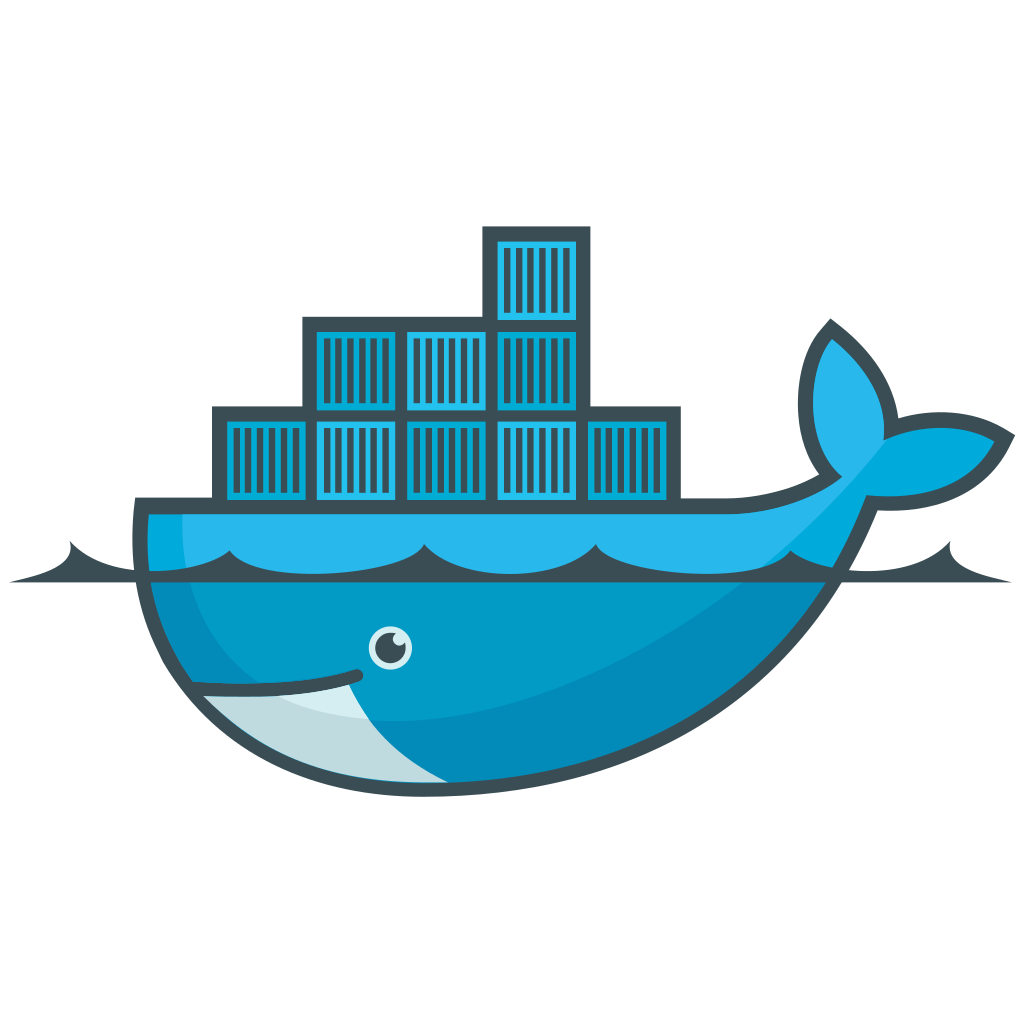
\includegraphics[height=1.6cm]{figures/logo_docker.png}
\end{tabular}
\caption{Technology stack overview.}\label{fig:tech-logos}
\end{figure}

\subsection{Backend}

\textbf{NestJS}~\cite{nestjs} (version~11) is the backend framework. It was chosen because its
modular architecture enforces a clear structure at the framework level --- exactly what a
ten-domain monolith needs to stay maintainable. Its decorator-based approach to routing,
dependency injection, guards, and Swagger documentation fits naturally with the four-layer
convention adopted across the project.

\textbf{Prisma}~\cite{prisma} (version~7) serves as the ORM and database access layer. Its
typed client, generated from a declarative schema, provides compile-time safety on every query.
The multi-file schema support (15 files) keeps the 55-model schema organized by domain, and
\texttt{prisma migrate deploy} provides idempotent, production-safe migrations.

\textbf{Google Gemini}~\cite{gemini} provides both the embedding model and the generation model
for the AI copilot. Using a managed API avoided installing and operating a self-hosted
inference stack during a time-limited internship. Gemini's \texttt{flash-lite} variant serves
as a cheap, fast reranking model on its own quota bucket.

\subsection{Frontend}

\textbf{Next.js}~\cite{nextjs} (version~16, App Router) is the frontend framework. Its
file-based routing, built-in internationalization support through next-intl, and React Server
Components provide the foundation for a bilingual, authenticated single-page application.

\textbf{React}~\cite{react} (version~19) is the UI runtime. Combined with TanStack
Query~\cite{tanstackquery} for server-state caching and Zustand~\cite{zustand} for lightweight
client state, it provides a clean separation between data fetching, UI state, and rendering.

\textbf{Tailwind CSS}~\cite{tailwindcss} (version~4) with Radix UI primitives (shadcn pattern)
handles styling. Utility-first CSS keeps styles co-located with components, and Radix provides
accessible, unstyled UI primitives that are customized to the platform's design.

\subsection{Database and infrastructure}

\textbf{PostgreSQL}~\cite{postgresql} (version~15) with the \textbf{pgvector}~\cite{pgvector}
extension is the single datastore backing both the transactional domain and the RAG vector
store. This choice keeps the system simple: because the embeddings are stored in the same
database as the domain data, retrieval can be permission-scoped in plain SQL, and there is no
separate vector database to operate, synchronize, or secure.

\textbf{Redis}~\cite{redis} was evaluated for the two jobs it is usually brought in to do here
--- caching and distributed locking --- and deliberately not adopted. The locking requirement is
real: the platform runs a dozen per-minute cron jobs, and in a replicated deployment each must
execute exactly once. PostgreSQL already answers that with \texttt{SELECT ... FOR UPDATE SKIP
LOCKED}, which gives the same mutual exclusion with crash-safe expiry and no second datastore to
deploy, secure, monitor, and keep consistent with the first. Caching was not adopted either,
because the query volume of an agency of roughly seven people does not yet justify the
invalidation complexity that a cache introduces. The rule applied throughout this chapter is to
add infrastructure when a measured problem requires it, not in anticipation; if read volume
later grows enough to warrant a cache, Redis is the natural addition, and the lock implementation
is already isolated behind a service that could adopt it without touching the callers.

\textbf{Docker}~\cite{docker} provisions the local infrastructure via \texttt{docker-compose}:
PostgreSQL (with pgvector) and Mailpit (development SMTP). Each application ships its
own Dockerfile as a reproducible build recipe.

\subsection{AI and retrieval}

The AI subsystem uses \textbf{Retrieval-Augmented Generation
(RAG)}~\cite{lewis2020rag} --- rather than sending questions directly to a language model, it
first retrieves the most relevant project content from the vector store, then asks the model to
generate an answer grounded in and cited to that content. The retrieval pipeline combines
\textbf{vector search} (cosine similarity over pgvector HNSW indexes) with \textbf{lexical
search} (PostgreSQL full-text search over GIN-indexed tsvector columns), fused by
\textbf{Reciprocal Rank Fusion}~\cite{cormack2009rrf}. An optional LLM reranker re-orders the
fused results. The full pipeline is the subject of Chapter~5.

\subsection{Development tools}

The project uses \textbf{Git} for version control in a single repository holding both
applications. API documentation is auto-generated by \textbf{Swagger}~\cite{swagger} at
\texttt{/api}: every controller's endpoints, DTOs, and required permissions are browsable and
testable from one page (Figure~\ref{fig:swagger}). Form validation is built on
\textbf{Zod}~\cite{zod} schema factories that export
inferred TypeScript types, binding form values, the react-hook-form resolver, and the request
shape to one definition. \textbf{Firebase Cloud Messaging}~\cite{fcm} delivers push
notifications to users' devices.

\reportscreenshot{figures/screenshot_swagger}{Swagger UI at \texttt{/api}: the REST API's 20 controller groups with their documented endpoints.}{swagger}

\section{Testing Strategy}

Each sprint in Chapters~3 to~5 reports its own validation. This section states the strategy
those per-sprint sections are instances of, so the reasoning is given once rather than repeated
six times. Four techniques are used, each chosen for the kind of defect it is good at catching
(Table~\ref{tab:test-strategy}).

\begin{table}[H]
\centering
\caption{Testing techniques and what each is used for.}\label{tab:test-strategy}
\begin{tabular}{@{}>{\raggedright\arraybackslash}p{0.20\textwidth}>{\raggedright\arraybackslash}p{0.44\textwidth}>{\raggedright\arraybackslash}p{0.26\textwidth}@{}}
\tableheaderrow
\thcell{Technique} & \thcell{What it verifies} & \thcell{Where applied} \\
\midrule
Unit tests (Jest, mocked repositories) & Business rules and authorization branches in isolation --- the paths where a service decides who may do what. & Domain services and controllers, and the shared delivery channels \\
\midrule
End-to-end tests (supertest, live app) & That the RBAC catalogue behaves as declared once guards, services and the database are wired together --- the contract no unit test can prove. & The permission matrix across CEO, PM, PO, Scrum Master and engineer roles \\
\midrule
Property-based tests (fast-check + vitest) & Invariants that must hold over \emph{all} inputs rather than a few examples --- no task lost when the board regroups, casters surviving a round trip. & 13 client-side suites over the transform and parsing layers \\
\midrule
Offline evaluation harness & Quality of a component whose output is not a fixed expected value, so it must be measured statistically rather than asserted. & The AI subsystem: retrieval, answer quality, estimation (Chapter~5) \\
\bottomrule
\end{tabular}
\end{table}

The fourth row is what makes the AI subsystem different in kind. A CRUD endpoint either returns
the right row or it does not, so an assertion settles it. A retrieval pipeline has no single
correct output, so its quality has to be measured against gold sets and reported as a
distribution --- which is why Chapter~5 carries metrics where the other chapters carry acceptance
tables.

\textbf{Where the effort went.} The four techniques were applied where each buys the most
confidence per unit of effort. The authorization contract is the platform's highest-risk
surface, with 31 role types sharing one API, so it is covered end to end rather than by unit
tests, because only a live run through guards, services and the database proves the catalogue
behaves as declared. The transform and parsing layers are covered by property-based tests, since
their invariants are universally quantified and example-based tests would under-sample them. The
AI subsystem is measured statistically, because it is the one component whose output cannot be
asserted against a fixed expected value. Extending automated coverage further, by deepening
backend behavioural tests across the remaining domain modules, is listed as prioritized future
work in Annex~A.

\section{Risks and Technical Challenges}

Several risks and challenges were identified at the design stage and shaped the technical
decisions described above.

\begin{itemize}
  \item \textbf{AI hallucinations.} A language model asked about the company's projects without
    grounding will invent plausible answers. This is the central risk of the AI feature
    and the reason for adopting RAG: the model only sees retrieved, permission-scoped project
    content, and a confidence gate refuses the question entirely when retrieval finds nothing
    relevant. The design principle is \emph{honesty over coverage}: refuse rather than guess.
  \item \textbf{Breadth versus consistency.} Covering ten operational domains in one codebase
    risks a large, inconsistent system. The mitigation is the strict four-layer, per-feature
    architecture enforced across every module, so that any domain follows the same structure
    once the pattern is learned.
  \item \textbf{No self-hosted ML infrastructure.} Installing and operating a GPU-backed
    inference stack was not feasible within the internship timeline. Using Google Gemini as a
    managed API avoided this, at the cost of an external dependency and its rate limits.
  \item \textbf{Security across a rich role model.} With approximately 31 role types sharing one
    API, the risk of authorization gaps is high. The mitigation is a centralized RBAC catalogue
    (approximately 120 permissions mapped in one constant) applied by a single guard on every
    route, with finer ownership checks done inside the services, where the data is available.
  \item \textbf{Integration complexity.} Multi-channel notifications (in-app, email, push,
    Telegram, ntfy), infrastructure health checks (ICMP, HTTP), and the AI indexing pipeline
    all involve asynchronous, cross-module orchestration. Distributed Postgres-based locking
    ensures that cron jobs run exactly once in a multi-instance deployment.
\end{itemize}

\section{Chapter Conclusion}

This chapter prepared the ground for the implementation chapters that follow. The project was
organized as a Scrum process with variable-length sprints, a 252-point product backlog
distributed across six sprints, and a strict dependency-driven plan. Eight non-functional
requirements --- security, data sovereignty, performance, reliability, maintainability,
internationalization, usability and portability --- constrain every feature in that backlog, and
most of the design decisions in this chapter exist to satisfy one of them. The architecture is a
two-application system --- a stateless NestJS API and a Next.js client --- backed by PostgreSQL
with pgvector, deliberately built as a modular monolith rather than a microservice
decomposition, and following a uniform four-layer convention that keeps ten domains
maintainable. The database schema comprises 55 models organized into eight entity families. The
technology choices were driven by type safety, maintainability, and the need to keep the AI
subsystem inside the same datastore as the domain, and the testing strategy pairs unit,
end-to-end, property-based and statistical evaluation to the kind of defect each catches.
Chapters~3 to~5 now describe the implementation sprint by sprint.
